\subsubsection*{Definition}

Decision trees are binary trees used for 
classification. Each tree consists of two 
types of components: internal nodes and leaves.

Each internal node has two children and contains
 a splitting function that determines whether 
 incoming data is passed to the left or right 
 child. The splitting function follows the 
 pattern:

\[
f_*({t_{\mathrm{start}}}^* , {t_{\mathrm{end}}}^*) \leq \tau^*
\]

where \( f_* \) is a chosen interval feature, 
\( ({t_{\mathrm{start}}}^*, {t_{\mathrm{end}}}^*) \) 
is the selected time interval, and \( \tau^* \) 
is a threshold.

In practice, this means each input is evaluated
on a specific interval using a particular 
feature. If the result is less than or equal
 to the threshold, the data is passed to the 
 left child; otherwise, it is passed to the 
 right child.

Leaves, the second component type, 
do not perform any splits. They assign a 
class label to any data that reaches them. 
Nodes may have either other nodes or leaves 
as children.


Let \(A\), \(B\), and \(C\) be class labels, and \(\alpha\), \(\beta\), \(\gamma\) denote the chosen parameters at each internal node. A decision tree can be visualized as follows:
\subsubsection*{Visualized Decision Tree}
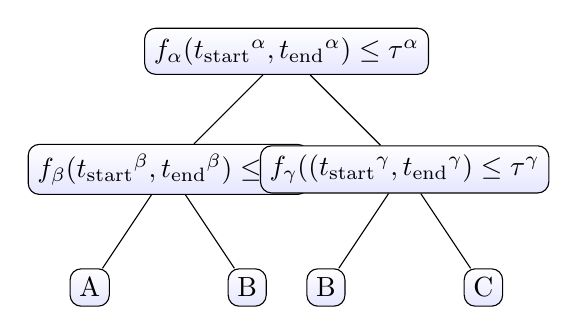
\begin{tikzpicture}[
    level 1/.style={sibling distance=30mm, level distance=15mm},
    level 2/.style={sibling distance=20mm, level distance=15mm},
    every node/.style = {shape=rectangle, rounded corners, draw, align=center, top color=white, bottom color=blue!10}
  ]
\node {\(f_{\alpha} ({t_{\mathrm{start}}}^{\alpha}, {t_{\mathrm{end}}}^\alpha) \leq \tau^{\alpha}\)}
  child {
    node {\(f_{\beta} ({t_{\mathrm{start}}}^{\beta}, {t_{\mathrm{end}}}^\beta) \leq \tau^{\beta}\)}
      child { node {A} }
      child { node {B} }
  }
  child {
    node {\(f_{\gamma} (({t_{\mathrm{start}}}^{\gamma}, {t_{\mathrm{end}}}^\gamma) \leq \tau^{\gamma}\)}
      child { node {B} }
      child { node {C} }
  };
\end{tikzpicture}

\subsubsection*{Random Forests}
To now classify a timeseries not just one tree is used. 
Multiple trees give their class prediciton, which is then 
aggregated and shown as a class probabilty. For this process to make sense
each tree should look at a diverse set of features. This is done by 
using a random sampling strategy in the training of each tree. 

The combination of many relatively uncorrelated trees can produce a forest whose prediction is more accurate than that of any of the individual trees. %% TODO: qutoe it from random forests